\begin{center}

{.}
  \vspace{1.2cm}

  \thispagestyle{empty}

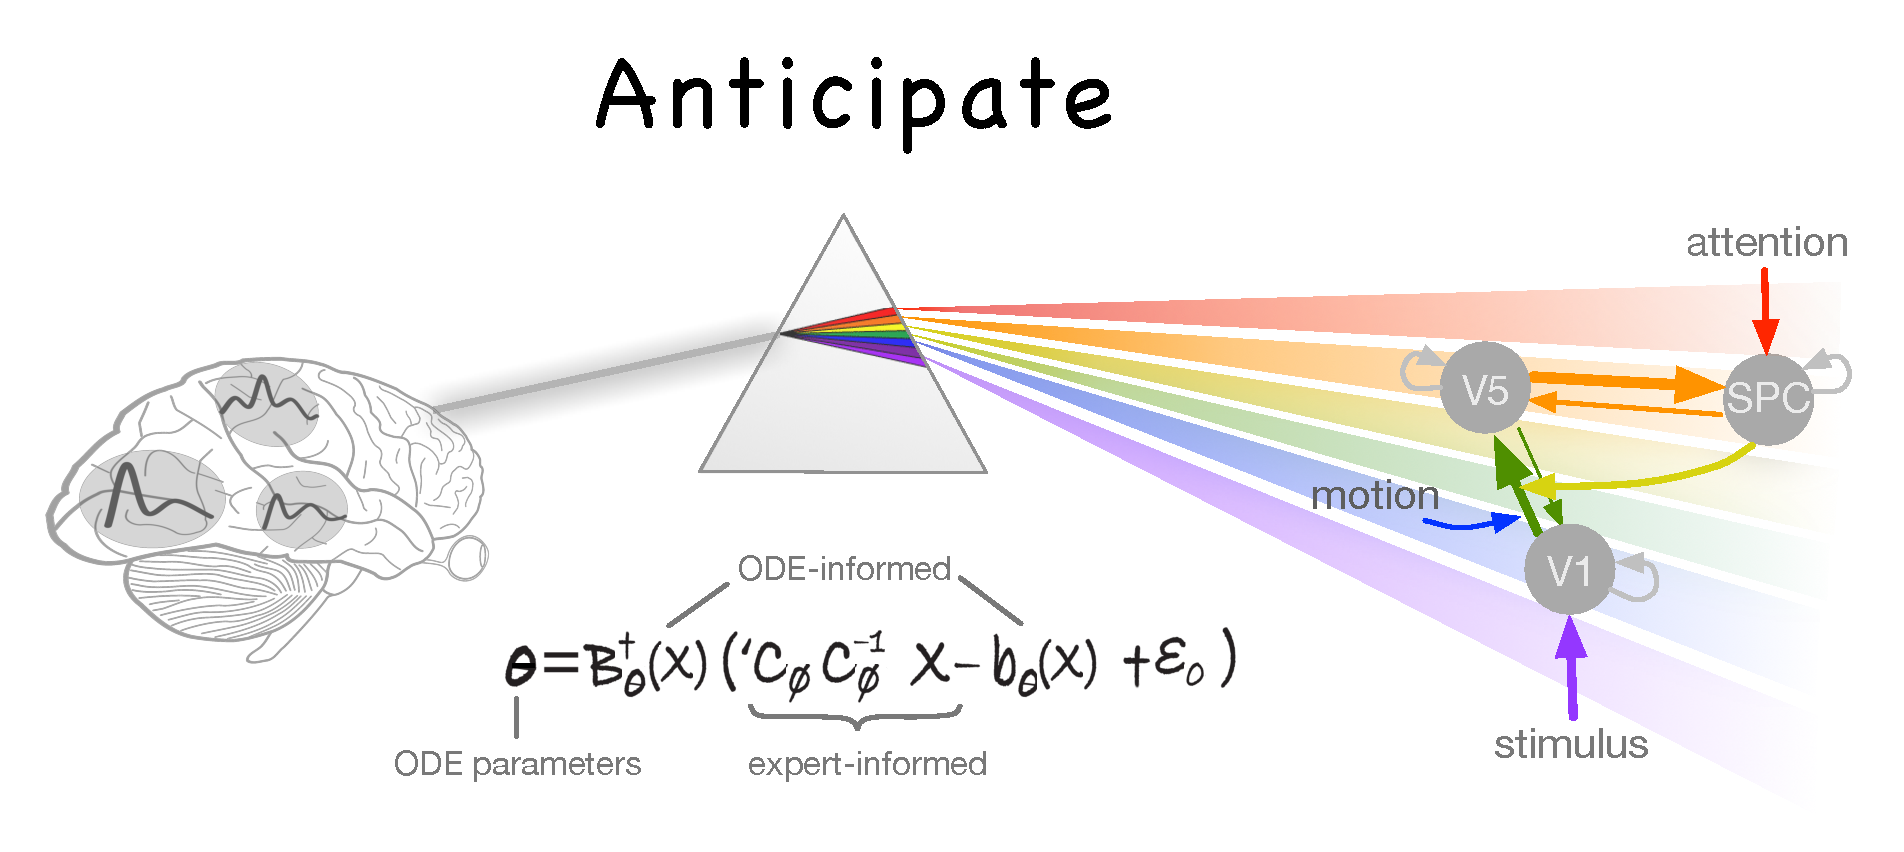
\includegraphics[width=5in]{logo.png}
\vspace{0.5cm}  

  {\LARGE\bf Code Documentation of Variational Gradient Matching \\ \vspace{0.3cm} for Dynamical Systems}
  
  \thispagestyle{empty}
             

%  Version of \today

  \vspace{1.2cm}

%\includegraphics[width=6in]{cover_pic.png}
\end{center}
\vspace{2cm}
 {\Large \textbf{Authors}:\vspace{0.4cm}
\newline \textbf{Nico Stephan Gorbach} and \textbf{Stefan Bauer}, email: nico.gorbach@gmail.com}

\vspace{2cm}
{{\Large\textbf{Contents}:}\vspace{0.4cm}
\newline Code documentation for Variational Gradient Matching (VGM) described in the NIPS (2018) paper \href{https://papers.nips.cc/paper/7066-scalable-variational-inference-for-dynamical-systems.pdf}{Scalable Variational Inference for Dynamical Systems} by Nico S. Gorbach, Stefan Bauer and Joachim M. Buhmann (arxiv paper: \href{https://arxiv.org/pdf/1705.07079.pdf}{https://arxiv.org/pdf/1705.07079.pdf}). Please cite our paper if you use our program for a further publication. The derivations in this document are also given in the doctoral thesis \href{https://www.research-collection.ethz.ch/handle/20.500.11850/261734}{https://www.research-collection.ethz.ch/handle/20.500.11850/261734} as well as in parts of Wenk et al. (2018). Matlab code is illustrated in \color{RoyalPurple} purple \color{black} and the console output is illustrated in \color{MidnightBlue} blue\color{black}.

\vspace{0.3cm}
The code is available at \url{https://github.com/ngorbach/Variational_Gradient_Matching_for_Dynamical_Systems}. Online documentation of this code is available at \url{https://ngorbach.github.io/Variational_Gradient_Matching_for_Dynamical_Systems/#17}. In the repository, run one of the Matlab scripts\newline \textit{VGM\textunderscore for\textunderscore Lotka\textunderscore Volterra.m}, \textit{VGM\textunderscore for\textunderscore Lorenz96.m} and \textit{VGM\textunderscore for\textunderscore Lorenz\textunderscore attractor.m}. Alternatively, one can also run the live scripts \textit{VGM\textunderscore for\textunderscore Lotka\textunderscore Volterra\textunderscore live\textunderscore script.mlx}, \textit{VGM\textunderscore for\textunderscore Lorenz96\textunderscore live\textunderscore script.mlx} or\newline \textit{VGM\textunderscore for\textunderscore Lorenz\textunderscore Attractor\textunderscore live\textunderscore script.mlx}. The Matlab symbolic toolbox is required for this code.}


